\documentclass[a4paper]{article}
\usepackage[english]{babel}
\usepackage[utf8]{inputenc}
\usepackage{textcomp}
\usepackage{amsmath}
\usepackage{amssymb}
\usepackage{gensymb}
\usepackage{physics}
\usepackage{graphicx}
\usepackage[colorinlistoftodos]{todonotes}
\usepackage{xcolor}
\usepackage{array}
\usepackage{tabularx}
\usepackage{tikz}
\usepackage{pgfplots}
\usepackage{framed}
\usepackage{xfrac}
\usepackage[most]{tcolorbox}
\usepackage{fix-cm}
\usepackage{cancel}
\usepackage[margin=0.5in]{geometry}
\usetikzlibrary{quotes,angles}
\usetikzlibrary{decorations.pathreplacing}
\usetikzlibrary{calc}
\usepgfplotslibrary{fillbetween}

\let\phi\varphi
\let\bf\textbf
\let\la\langle
\let\ra\rangle
\colorlet{shadecolor}{orange!15}
\pgfplotsset{compat=1.18}
\newcommand\der[2]{\frac{d #1}{d #2}}
\newcommand\Deltat{\Delta t}
\newcommand{\AxisRotator}[1][rotate=0]{%
    \tikz [x=0.25cm,y=0.60cm,line width=.2ex,-stealth,#1] \draw (0,0) arc (-150:150:1 and 1);%
}
\def\centerarc[#1](#2)(#3:#4:#5){\draw[#1] ($(#2)+({#5*cos(#3)},{#5*sin(#3)})$) arc (#3:#4:#5)}
% Syntax: \centerarc[draw options] (center) (initial angle:final angle:radius);

\title{Vectors in Space}
\author{OpenStax Calculus Vol. 3}
\date{}

\begin{document}
\setcounter{section}{2}
\maketitle

\subsection{Vectors in the Plane}
A vector in a plane is represented by a directed line section, its endpoints are called the initial and terminal points respectively. An arrow from the initial point to the terminal point indicates the direction of the vector and the length of the line segment represents its magnitude. The notation $||\vec{v}||$ or $||\bf{v}||$ is used to denote the magnitude of the vector $\vec{v}$ (or \bf{v}). The zero vector is a vector with the same initial and terminal point denoted $\vec{0}$ or \bf{0}. 
\vspace{1mm}\\
Vectors with the same magnitude and direction are considered equivalent vectors and are treated as equal even if they have different initial points. Two vectors are parallel if they have the same or opposite directions. Vectors are defined by magnitude and direction regardless of the location of the initial point.
\vspace{2mm}\\
\bf{Combining Vectors}\vspace{2mm}\\
Scalars are quantities that have only a magnitude and no direction. Multiplying a vector by a scalar changes the vector's magnitude; this is called scalar multiplication. Changing the magnitude of a vector does not indicate a change in its direction.
\begin{shaded}
    \noindent\underline{\bf{Definition of Scalar Multiplication}}\vspace{2mm}\\
    The product $k\vec{v}$ of a vector $\vec{v}$ and scalar $k$ is a vector with a magnitude that is $|k| \cdot ||\vec{v}||$ and a direction that is equal to the direction of $\vec{v}$ if $k>0$ and opposite the direction of $\vec{v}$ if $k<0$. If $k = 0$ or $\vec{v} = \vec{0} \implies k\vec{v} = \vec{0}$
\end{shaded}
\noindent Because each vector may have its own direction, the process for adding vectors is different from adding scalars. The most common graphical method for adding two vectors is to place the initial point of the second vector at the terminal point of the first. The sum of the vectors $\vec{v}$ and $\vec{w}$ is the vector with an initial point that coincides with the initial point of $\vec{v}$ and a terminal point that coincides with the terminal point of $\vec{w}$.
\begin{center}
    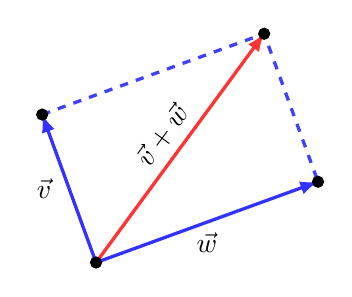
\begin{tikzpicture}[scale=2]
        \draw (0,0) coordinate (a);
        \draw ({1.5*cos(20)},{1.5*sin(20)}) coordinate (b);
        \draw ({cos(110)},{sin(110)}) coordinate (c);
        \draw ({1.5*cos(20) + cos(110)},{1.5*sin(20) + sin(110)})coordinate (d);
        \draw[dashed,very thick,white!25!blue] (c)--(d)--(b);
        \draw[->,very thick,-latex,white!20!blue] (a)--node[left,color=black,xshift=-0.25em]{$\vec{v}$}(c);
        \draw[->,very thick,-latex,white!20!blue] (a)--node[below,color=black]{$\vec{w}$}(b);
        \draw[->,very thick,-latex,white!20!red] (a)--node[above,color=black,rotate=53.69]{$\vec{v} + \vec{w}$}(d);
        \filldraw[black] (a) circle (1pt);
        \filldraw[black] (b) circle (1pt);
        \filldraw[black] (c) circle (1pt);
        \filldraw[black] (d) circle (1pt);
    \end{tikzpicture}
    \hspace{1.5cm}
    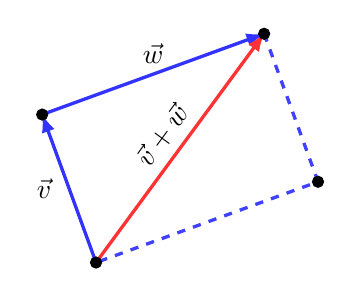
\begin{tikzpicture}[scale=2]
        \draw (0,0) coordinate (a);
        \draw ({1.5*cos(20)},{1.5*sin(20)}) coordinate (b);
        \draw ({cos(110)},{sin(110)}) coordinate (c);
        \draw ({1.5*cos(20) + cos(110)},{1.5*sin(20) + sin(110)})coordinate (d);
        \draw[dashed,very thick,white!25!blue] (d)--(b)--(a);
        \draw[->,very thick,-latex,white!20!blue] (a)--node[left,color=black,xshift=-0.25em]{$\vec{v}$}(c);
        \draw[->,very thick,-latex,white!20!blue] (c)--node[above,color=black]{$\vec{w}$}(d);
        \draw[->,very thick,-latex,white!20!red] (a)--node[above,color=black,rotate=53.69]{$\vec{v} + \vec{w}$}(d);
        \filldraw[black] (a) circle (1pt);
        \filldraw[black] (b) circle (1pt);
        \filldraw[black] (c) circle (1pt);
        \filldraw[black] (d) circle (1pt);
    \end{tikzpicture}
\end{center}
For $\vec{u} = \vec{v} + \vec{w}$, the initial point of $\vec{u}$ is the initial point of $\vec{v}$ and the terminal point is the terminal point of $\vec{w}$. These three vectors form a triangle, it follows that the length of any one side is less than the sum of the lengths of the remaining sides, therefore: $||\vec{u}|| \leq ||\vec{v}|| + ||\vec{w}||$
\vspace{1mm}\\
For vector subtraction, $\vec{v} - \vec{w}$ is defined as $\vec{v} + (-\vec{w}) = \vec{v} + (-1)\vec{w}$. The vector $\vec{v} - \vec{w}$ is called the vector difference and is depicted graphically by drawing a vector from the terminal point of $\vec{w}$ to the terminal point of $\vec{v}$.
\begin{center}
    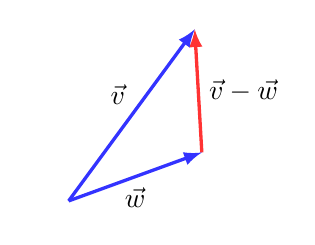
\begin{tikzpicture}[scale=1.5]
        \draw (0,0) coordinate (a);
        \draw ({1.2*cos(20)},{1.2*sin(20)}) coordinate (b);
        \draw ({cos(110)},{sin(110)}) coordinate (c);
        \draw ({1.5*cos(20) + cos(110)},{1.5*sin(20) + sin(110)})coordinate (d);
        \draw[->,very thick,-latex,white!20!red] (b)--node[right,color=black]{$\vec{v} - \vec{w}$}(d);
        \draw[->,very thick,-latex,white!20!blue] (a)--node[below,color=black]{$\vec{w}$} (b);
        \draw[->,very thick,-latex,white!20!blue] (a)--node[above,color=black,xshift=-0.5em]{$\vec{v}$}(d);
    \end{tikzpicture}
    \hspace{1.5cm}
    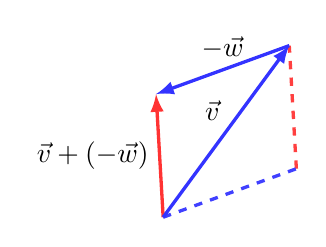
\begin{tikzpicture}[scale=1.5]
        \draw (0,0) coordinate (a);
        \draw ({1.2*cos(20)},{1.2*sin(20)}) coordinate (b);
        \draw ({(1.5*cos(20) + cos(110)) - (1.2*cos(20))},{(1.5*sin(20) + sin(110)) - (1.2*sin(20))}) coordinate (c);
        \draw ({1.5*cos(20) + cos(110)},{1.5*sin(20) + sin(110)})coordinate (d);
        \draw[dashed,very thick,white!25!red] (b)--(d);
        \draw[->,very thick,-latex,white!20!red] (a)--node[left,color=black]{$\vec{v}+ (-\vec{w})$}(c);
        \draw[dashed,very thick,white!25!blue] (a)--(b);
        \draw[->,very thick,-latex,white!20!blue] (a)--node[above,color=black,xshift=-0.5em]{$\vec{v}$}(d);
        \draw[->,very thick,-latex,white!20!blue] (d)--node[above,color=black]{$-\vec{w}$}(c);
    \end{tikzpicture}
\end{center}
\bf{Vector Components}\vspace{2mm}\\
A vector with initial point at the origin is called a standard-position vector. Because the initial point of any vector in standard position is (0,0), it can be described by the coordinates of its terminal point.
\begin{shaded}
    \noindent\underline{\bf{Definition}}
    \vspace{2mm}\\
    The vector with initial point (0,0) and terminal point $(x,y)$ can be written in component form as
    \begin{align*}
        \vec{v} = \la x,y \ra
    \end{align*}
    The scalars $x$ and $y$ are called the components of $\vec{v}$
\end{shaded}
\noindent For a vector not already in standard form its component form can be determined algebraically by subtracting the $x$ and $y$ values of the initial point from those of the terminal point.
\begin{shaded}
    \noindent Let $\vec{v}$ be a vector with initial point $(x_i,y_i)$ and terminal point $(x_t,y_t)$. Then $\vec{v}$ can be expressed in component form as 
    \begin{align*}
        \vec{v}= \la x_t - x_i, y_t - y_i \ra
    \end{align*}
\end{shaded}
\noindent To find the magnitude of a vector, calculate the distance between its initial and terminal points. The magnitude of vector $\vec{v} = \la x, y \ra$ is denoted $||\vec{v}||$ and can be calculated using the formula
\begin{align*}
    ||\vec{v}|| = \sqrt{x^2 + y^2}
\end{align*}
Based on this, it is clear that for any vector $\vec{v}$, $||\vec{v}|| \geq 0$, and $||\vec{v}|| = 0$ if and only if $\vec{v} = \vec{0}$.\vspace{1mm}\\
The magnitude of a vector can also be derived using Pythagorean theorem.
\begin{center}
    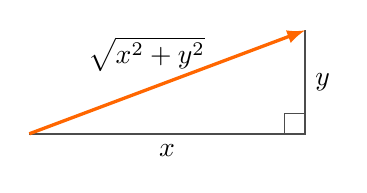
\begin{tikzpicture}[scale=1.75]
        \draw (0,0) coordinate (a);
        \draw (2,0) coordinate (b);
        \draw (2,0.75) coordinate (c);
        \draw[black!70] (1.85,0)--(1.85,0.15)--(2,0.15);
        \draw[thick,black!70] (a)--node[below,color=black]{$x$}(b)--node[right,color=black]{$y$}(c);
        \draw[->,very thick,-latex,red!20!orange] (a)--node[above,color=black,xshift=-0.75em]{$\sqrt{x^2 + y^2}$} (c); 
    \end{tikzpicture}
\end{center}
Expressing vectors in component form allows scalar multiplication and vector addition to be performed algebraically.
\begin{shaded}
    \noindent Let $\vec{v} = \la x_1, y_1 \ra$ and $\vec{w} = \la x_2,y_2 \ra$ be vectors, and let $k$ be a scalar.\vspace{1mm}\\
    \bf{Scalar Multiplication:} $k\vec{v} = \la kx_1, ky_1 \ra$\\
    \bf{Vector Addition:} $\vec{v} + \vec{w} = \la x_1,y_1 \ra + \la x_2,y_2 \ra = \la x_1 + x_2, y_1 + y_2 \ra$
\end{shaded}

\begin{shaded}
    \noindent\underline{\bf{Properties of Vector Operations}}\vspace{2mm}\\
    Let $\vec{u}, \vec{v}$, and $\vec{w}$ be vectors in a plane. Let $r$ and $s$ be scalars.
    \begin{align*}
        \text{i}&. &\vec{u} + \vec{v} &= \vec{v} + \vec{u} &\text{Commutative Property}\\
        \text{ii}&. &(\vec{u} + \vec{v}) + \vec{w} &= \vec{u} + (\vec{v} + \vec{w}) &\text{Associative Property}\\
        \text{ii}&. &\vec{u} + \vec{0} &= \vec{u} &\text{Additive Identity Property}\\
        \text{iv}&. &\vec{u} + (-\vec{u}) &= \vec{0} &\text{Additive Inverse Property}\\
        \text{v}&. &r(s\vec{u}) &= (rs)\vec{u} &\text{Associativity of Scalar Multiplication}\\
        \text{vi}&. &(r + s)\vec{u} &= r\vec{u} + s\vec{u} &\text{Distributive Property}\\
        \text{vii}&. &r(\vec{u} + \vec{v}) &= r\vec{u} + r\vec{v} &\text{Distributive Property}\\
        \text{viii}&. &1\vec{u} &= \vec{u} &\text{Identity Property}\\
        \text{ix}&. &0u &= \vec{0} &\text{Zero Property}
    \end{align*}
\end{shaded}
\begin{shaded}
    \noindent\underline{\bf{Proof of Commutative \& Distributive Properties}}
    \vspace{2mm}\\
    Let $\vec{u} = \la x_1, y_1 \ra$ and $\vec{v} = \la x_2, y_2 \ra$
    \vspace{1mm}\\
    \bf{Commutative Property}
    \vspace{1mm}\\
    Apply the commutative property for $\mathbb{R}$
    \begin{align*}
        \vec{u} + \vec{v} = \la x_1 + x_2, y_1 + y_2 \ra = \la x_2 + x_1, y_2 + y_1 \ra = \vec{v} + \vec{u}
    \end{align*}
    \bf{Distributive Property}
    \vspace{1mm}\\
    Apply the distributive property for $\mathbb{R}$
    \begin{align*}
        r(\vec{u} + \vec{v}) &= r \cdot \la x_1 + x_2, y_1 + y_2 \ra\\
        &= \la r(x_1 + x_2), r(y_1 + y_2) \ra\\
        &= \la rx_1 + rx_2, ry_1 + ry_2 \ra\\
        &= \la rx_1, ry_1 \ra + \la rx_2, ry_2 \ra\\
        &= r\vec{u} + r\vec{v}
    \end{align*}
\end{shaded}

\end{document}